\section{ Comparison With Previous Work}
\label{sec:app-comparison}

In this section, we provide a direct comparison, illustrated in Figure~\ref{fig:comparison_2016}, between our results (Figure~\ref{fig:3PC}) and those from the prior 2016 work by Hooper and Linden~\cite{Hooper:2016rap}. Their analysis was based on 7 years of Fermi data, in contrast to the 15.8 years of data utilized in our work. The 2016 study favored an MSP gamma-ray luminosity function with parameters of $\langle L_{\gamma} \rangle \sim (0.7-6) \times 10^{34} \, \textrm{erg/s}$ and $\sigma_L \sim 1-3$.

While our results are statistically consistent with theirs at the $\sim 2\sigma$ level, our analysis prefers smaller values for $\langle L_{\gamma} \rangle$ and larger values for $R_\textrm{MSP}$ by a factor of $\sim 2-8$. Furthermore, although the best-fit values for both distributions lie near the $N_{MSP}=30$ curve, our findings suggest a narrower range of $N_{MSP} \sim 17 - 37$, compared to the previous estimate of $N_{MSP} \sim 12 - 50$. Our updated analysis refines the prior work by both encompassing the findings of Ref.~\cite{Hooper:2016rap} as far as $N_{MSP}$ is concerned, and providing tighter constraints on the number of MSPs required to explain the Galactic Center Excess.




\begin{figure}
    \centering
    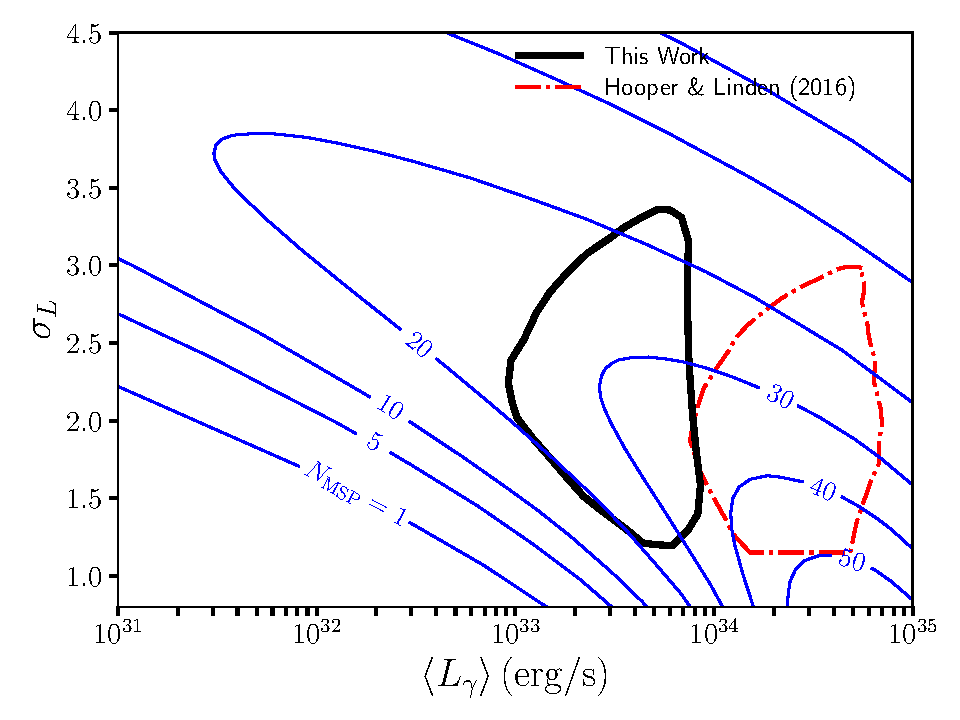
\includegraphics[width=0.5\linewidth]{img/comparison_2016.pdf}
    \caption{ As in Figure \ref{fig:3PC}, for the $2\sigma$ contours, but comparing the results from the prior 2016 work from Hooper and Linden \cite{Hooper:2016rap} with our most recent findings.}
    \label{fig:comparison_2016}
\end{figure}

